\documentclass[10pt]{article}
\usepackage[utf8]{inputenc}
\usepackage[T1]{fontenc}
\usepackage{amsmath}
\usepackage{amsfonts}
\usepackage{amssymb}
\usepackage[version=4]{mhchem}
\usepackage{stmaryrd}
\usepackage{graphicx}
\usepackage[export]{adjustbox}
\graphicspath{ {./images/} }

\begin{document}
\section*{PHYSICS}
\section*{SECTION-A}
\begin{enumerate}
  \item The electric potential at the centre of two concentric half rings of radii \(R_{1}\) and \(R_{2}\), having same linear charge density \(\lambda\) is\\
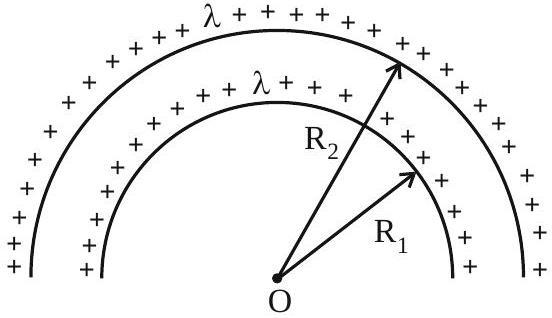
\includegraphics[max width=\textwidth, center]{2025_10_02_fdf5c730b8a604381ef3g-1}\\
(1) \(\frac{2 \lambda}{\epsilon_{0}}\)\\
(2) \(\frac{\lambda}{2 \epsilon_{0}}\)\\
(3) \(\frac{\lambda}{4 \epsilon_{0}}\)\\
(4) \(\frac{\lambda}{\epsilon_{0}}\)
\end{enumerate}

Official Ans. by NTA (2)\\
Allen Ans. (2)\\
Sol. Potential at centre\\
\(\mathrm{V}=\frac{\left(\lambda \cdot \pi \mathrm{R}_{2}\right)}{4 \pi \varepsilon_{0} \mathrm{R}_{2}}+\frac{\left(\lambda \cdot \pi \mathrm{R}_{1}\right)}{4 \pi \varepsilon_{0} \mathrm{R}_{1}}\)\\
\(=\frac{\lambda}{2 \varepsilon_{0}}\)\\
2. Let \(\gamma_{1}\) be the ratio of molar specific heat at constant pressure and molar specific heat at constant volume of a monoatomic gas and \(\gamma_{2}\) be the similar ratio of diatomic gas. Considering the diatomic gas molecule as a rigid rotator, the ratio, \(\frac{\gamma_{1}}{\gamma_{2}}\) is\\
(1) \(\frac{27}{35}\)\\
(2) \(\frac{35}{27}\)\\
(3) \(\frac{25}{21}\)\\
(4) \(\frac{21}{25}\)

Official Ans. by NTA (3)\\
Allen Ans. (3)\\
Sol. For monoatomic gas \(\gamma_{1}=\frac{5}{3}\)\\
For diatomic gas at low temperatures\\
\(\gamma_{2}=\frac{7}{5}\)\\
\(\therefore \frac{\gamma_{1}}{\gamma_{2}}=\frac{\frac{5}{3}}{\frac{7}{5}}=\frac{25}{21}\)

\section*{TEST PAPER WITH SOLUTION}
\begin{enumerate}
  \setcounter{enumi}{2}
  \item An \(\alpha\)-particle, a proton and an electron have the same kinetic energy. Which one of the following is correct in case of their De-Broglie wavelength:\\
(1) \(\lambda_{\alpha}>\lambda_{\mathrm{p}}>\lambda_{\mathrm{e}}\)\\
(2) \(\lambda_{\alpha}<\lambda_{\mathrm{p}}<\lambda_{\mathrm{e}}\)\\
(3) \(\lambda_{\alpha}=\lambda_{\mathrm{p}}=\lambda_{\mathrm{e}}\)\\
(4) \(\lambda_{\alpha}>\lambda_{\mathrm{p}}<\lambda_{\mathrm{e}}\)
\end{enumerate}

Official Ans. by NTA (2)\\
Allen Ans. (2)\\
Sol. \(\quad \lambda_{\mathrm{D}}=\frac{\mathrm{h}}{\mathrm{p}}=\frac{\mathrm{h}}{\sqrt{2 \mathrm{mK}}}\)\\
\(\therefore \lambda \propto \frac{1}{\sqrt{\mathrm{~m}}}\)\\
\(\because \mathrm{m}_{\alpha}>\mathrm{m}_{\mathrm{p}}>\mathrm{m}_{\mathrm{e}}\)\\
\(\lambda_{e}>\lambda_{p}>\lambda_{\alpha}\)\\
4. If the distance of the earth from Sun is \(1.5 \times 10^{6}\) km. Then the distance of an imaginary planet from Sun, if its period of revolution is 2.83 years is:\\
(1) \(6 \times 10^{7} \mathrm{~km}\)\\
(2) \(6 \times 10^{6} \mathrm{~km}\)\\
(3) \(3 \times 10^{6} \mathrm{~km}\)\\
(4) \(3 \times 10^{7} \mathrm{~km}\)

Official Ans. by NTA (3)\\
Allen Ans. (3)\\
Sol. \(\mathrm{T}^{2} \propto \mathrm{R}^{3} \Rightarrow\left(\frac{\mathrm{~T}_{1}}{\mathrm{~T}_{2}}\right)^{2}=\left(\frac{\mathrm{R}_{1}}{\mathrm{R}_{2}}\right)^{3}\)\\
\(\Rightarrow\left(\frac{1}{2.83}\right)^{2}=\left(\frac{1.5 \times 10^{6}}{\mathrm{R}_{2}}\right)^{3}\)\\
\(\Rightarrow R_{2}=\left[(2.83)^{2} \times\left(1.5 \times 10^{6}\right)^{3}\right]^{1 / 3}\)\\
\(=8^{1 / 3} \times 1.5 \times 10^{6}=3 \times 10^{6} \mathrm{~km}\)\\
5. Match List I with List II

\begin{center}
\begin{tabular}{|l|l|l|l|}
\hline
\multicolumn{2}{|c|}{LIST I} & \multicolumn{2}{c|}{LIST II} \\
\hline
A. & AM Broadcast & I. & \(88-108 \mathrm{MHz}\) \\
\hline
B. & FM Broadcast & II. & \(540-1600 \mathrm{kHz}\) \\
\hline
C, & Television & III. & \(3.7-4.2 \mathrm{GHz}\) \\
\hline
D. & Satellite Communication & IV. & \(54 \mathrm{MH}_{\mathrm{z}}-590 \mathrm{MHz}\) \\
\hline
\end{tabular}
\end{center}

Choose the correct answer from the options given below:\\
(1) A-II, B-I, C-IV, D-III\\
(2) A-IV, B-III, C-I, D-II\\
(3) A-II, B-III, C-I, D-IV\\
(4) A-I, B-III, C-II, D-IV

Official Ans. by NTA (1)\\
Allen Ans. (1)\\
Sol. AM Broadast \(\rightarrow 540-1600 \mathrm{KHz}\)\\
FM Broadcast \(\rightarrow 88-108 \mathrm{MHz}\)\\
Television \(\rightarrow 54-890 \mathrm{MHz}\)\\
Salellite communication \(\rightarrow 3.7-4.2 \mathrm{GHz}\)\\
\(\therefore\) A-II, B-I, C-IV, D-III\\
6. The logic gate equivalent to the given circuit diagram is :\\
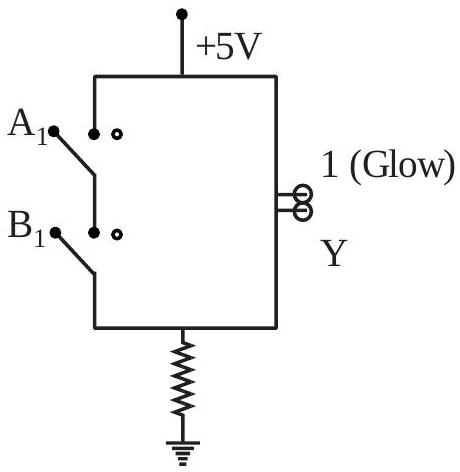
\includegraphics[max width=\textwidth, center]{2025_10_02_fdf5c730b8a604381ef3g-2(1)}\\
(1) OR\\
(2) NAND\\
(3) NOR\\
(4) AND

Official Ans. by NTA (2)\\
Allen Ans. (2)

Sol.

\begin{center}
\begin{tabular}{|c|c|c|}
\hline
\(\mathrm{A}_{1}\) & \(\mathrm{~B}_{1}\) & Y \\
\hline
0 & 0 & 1 \\
\hline
0 & 1 & 1 \\
\hline
1 & 0 & 1 \\
\hline
1 & 1 & 0 \\
\hline
\end{tabular}
\end{center}

\(\mathrm{Y}=\mathrm{A}_{1} \odot \mathrm{~B}_{1}\) NAND\\
7. A long solenoid is formed by winding 70 turns \(\mathrm{cm}^{-1}\). If 2.0 A current flows, then the magnetic field produced inside the solenoid is \(\_\_\_\_\) ( \(\mu_{0}=4 \pi \times 10^{-7} \mathrm{TmA}^{-1}\) )\\
(1) \(1232 \times 10^{-4} \mathrm{~T}\)\\
(2) \(176 \times 10^{-4} \mathrm{~T}\)\\
(3) \(352 \times 10^{-4} \mathrm{~T}\)\\
(4) \(88 \times 10^{-4} \mathrm{~T}\)

Official Ans. by NTA (2)\\
Allen Ans. (2)\\
Sol. \(B=\mu_{0} n I\)\\
\(=4 \pi \times 10^{-7} \times 70 \times 10^{2} \times 2\)\\
\(=56 \pi \times 10^{-4} \mathrm{~T}\)\\
\(=176 \times 10^{-4} \mathrm{~T}\)\\
8. Given below are two statements:

Statement I: Acceleration due to earth's gravity decreases as you go 'up' or 'down' from earth's surface.

Statement II: Acceleration due to earth's gravity is same at a height ' \(h\) ' and depth ' \(d\) ' from earth's surface, if \(\mathrm{h}=\mathrm{d}\).

In the light of above statements, choose the most appropriate answer form the options given below\\
(1) Statement I is incorrect but statement II is correct\\
(2) Both Statement I and Statement II are incorrect\\
(3) Statement I is correct but statement II is incorrect\\
(4) Both Statement I and II are correct

Official Ans. by NTA (3)\\
Allen Ans. (3)\\
Sol. \(g^{\prime}=\frac{g}{\left(1+\frac{h}{R}\right)^{2}}\)\\
\(\mathrm{g}^{\prime}=\mathrm{g}\left\{1-\frac{\mathrm{d}}{\mathrm{R}}\right\}\)\\
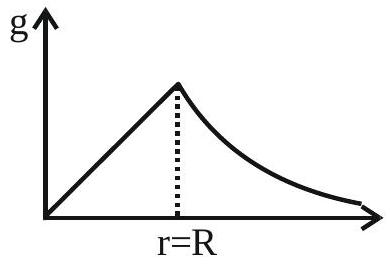
\includegraphics[max width=\textwidth, center]{2025_10_02_fdf5c730b8a604381ef3g-2}

Statement I is correct \& Statement II is incorrect\\
9. A metallic rod of length ' \(L\) ' is rotated with an angular speed of ' \(\omega\) ' normal to a uniform magnetic field ' B ' about an axis passing through one end of rod as shown in figure. The induced emf will be :\\
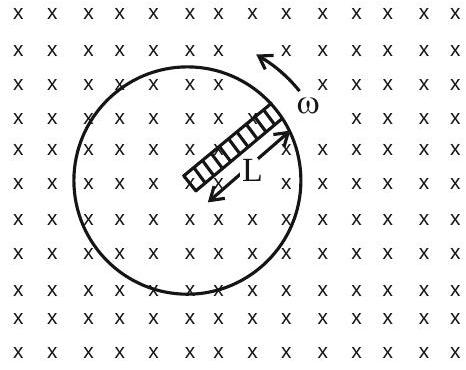
\includegraphics[max width=\textwidth, center]{2025_10_02_fdf5c730b8a604381ef3g-3}\\
(1) \(\frac{1}{4} \mathrm{~B}^{2} \mathrm{~L} \omega\)\\
(2) \(\frac{1}{4} \mathrm{BL}^{2} \omega\)\\
(3) \(\frac{1}{2} \mathrm{BL}^{2} \omega\)\\
(4) \(\frac{1}{2} \mathrm{~B}^{2} \mathrm{~L}^{2} \omega\)

Official Ans. by NTA (3)\\
Allen Ans. (3)

Sol.\\
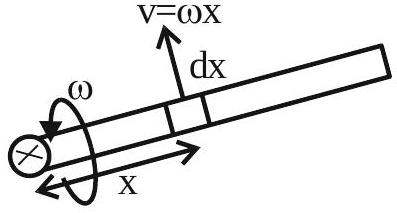
\includegraphics[max width=\textwidth, center]{2025_10_02_fdf5c730b8a604381ef3g-3(2)}\\
\(\int \mathrm{d} \varepsilon=\int \mathrm{B}(\omega \mathrm{x}) \mathrm{dx}\)\\
\(\varepsilon=\mathrm{B} \omega \int_{0}^{\mathrm{L}} \mathrm{xdx}=\frac{\mathrm{B} \omega \mathrm{L}^{2}}{2}\)\\
10. When a beam of white light is allowed to pass through convex lens parallel to principal axis, the different colours of light converge at different point on the principle axis after refraction. This is called :\\
(1) Scattering\\
(2) Chromatic aberration\\
(3) Spherical aberration\\
(4) Polarisation

Official Ans. by NTA (2)\\
Allen Ans. (2)\\
Sol. Based on fact.\\
11. The frequency ( \(v\) ) of an oscillating liquid drop may depend upon radius ( \(r\) ) of the drop, density ( \(\rho\) ) of liquid and the surface tension (s) of the liquid as :\\
\(v=r^{a} \rho^{b} s^{c}\). The values of \(a, b\) and \(c\) respectively are\\
(1) \(\left(-\frac{3}{2},-\frac{1}{2}, \frac{1}{2}\right)\)\\
(2) \(\left(\frac{3}{2},-\frac{1}{2}, \frac{1}{2}\right)\)\\
(3) \(\left(\frac{3}{2}, \frac{1}{2},-\frac{1}{2}\right)\)\\
(4) \(\left(-\frac{3}{2}, \frac{1}{2}, \frac{1}{2}\right)\)

Official Ans. by NTA (1)\\
Allen Ans. (1)\\
Sol. \(\quad\left[\mathrm{T}^{-1}\right]=\left[\mathrm{L}^{1}\right]^{\mathrm{a}}\left[\mathrm{M}^{1} \mathrm{~L}^{-3}\right]^{\mathrm{b}}\left[\frac{\mathrm{MLT}^{-2}}{\mathrm{~L}}\right]^{\mathrm{c}}\)\\
\(\Rightarrow \mathrm{T}^{-1}=\mathrm{M}^{\mathrm{b}+\mathrm{c}} \cdot \mathrm{L}^{\mathrm{a}-3 \mathrm{~b}} \cdot \mathrm{~T}^{-2 \mathrm{c}}\)\\
\(\mathrm{c}=\frac{1}{2}, \mathrm{~b}=-\frac{1}{2}, \quad \mathrm{a}-3 \mathrm{~b}=0\)\\
\(\mathrm{a}+\frac{3}{2}=0 \Rightarrow \mathrm{a}=-\frac{3}{2}\)\\
12. A body of mass 200 g is tied to a spring of spring constant \(12.5 \mathrm{~N} / \mathrm{m}\), while the other end of spring is fixed at point O . If the body moves about O in a circular path on a smooth horizontal surface with constant angular speed \(5 \mathrm{rad} / \mathrm{s}\), then the ratio of extension in the spring to its natural length will be :\\
(1) \(1: 2\)\\
(2) \(1: 1\)\\
(3) \(2: 3\)\\
(4) \(2: 5\)

Official Ans. by NTA (3)\\
Allen Ans. (3)\\
Sol.\\
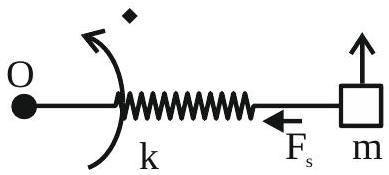
\includegraphics[max width=\textwidth, center]{2025_10_02_fdf5c730b8a604381ef3g-3(1)}

Natural length \(=\mathrm{L}_{0}\)\\
Extension \(=\mathbf{x}\)\\
\(\mathrm{kx}=\mathrm{m}\left(\mathrm{L}_{0}+\mathrm{x}\right) \omega^{2}\)\\
\(\Rightarrow 12.5 \mathrm{x}=\frac{1}{5}\left(\mathrm{~L}_{0}+\mathrm{x}\right) 25 \Rightarrow 1.5 \mathrm{x}=\mathrm{L}_{0}\)\\
\(\Rightarrow \frac{\mathrm{x}}{\mathrm{L}_{0}}=\frac{2}{3}\)\\
13. A cell of emf 90 V is connected across series combination of two resistors each of \(100 \Omega\) resistance. A voltmeter of resistance \(400 \Omega\) is used to measure the potential difference across each resistor. The reading of the voltmeter will be :\\
(1) 40 V\\
(2) 45 V\\
(3) 80 V\\
(4) 90 V

Official Ans. by NTA (1)\\
Allen Ans. (1)\\
Sol.\\
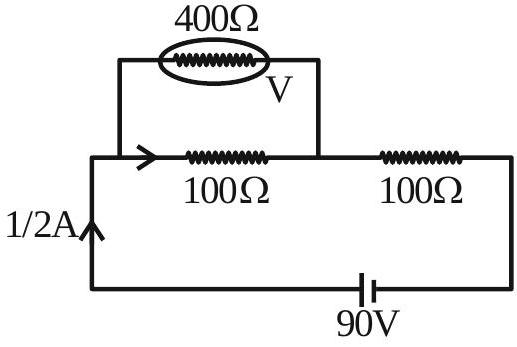
\includegraphics[max width=\textwidth, center]{2025_10_02_fdf5c730b8a604381ef3g-4}\\
\(R_{\text {eq }}=\frac{400 \times 100}{500}+100\)\\
\(=180 \Omega\)\\
\(\mathrm{i}=\frac{90}{180}=\frac{1}{2} \mathrm{~A}\)\\
Reading \(=\frac{1}{2} \times \frac{400}{500} \times 100\)\\
\(=40\) volt\\
14. The electric field and magnetic field components of an electromagnetic wave going through vacuum is described by\\
\(\mathrm{E}_{\mathrm{x}}=\mathrm{E}_{0} \sin (\mathrm{kz}-\omega \mathrm{t})\)\\
\(\mathrm{B}_{\mathrm{y}}=\mathrm{B}_{0} \sin (\mathrm{kz}-\omega \mathrm{t})\)\\
Then the correct relation between \(\mathrm{E}_{0}\) and \(\mathrm{B}_{0}\) is given by\\
(1) \(\mathrm{kE}_{0}=\omega \mathrm{B}_{0}\)\\
(2) \(\mathrm{E}_{0} \mathrm{~B}_{0}=\omega \mathrm{k}\)\\
(3) \(\omega \mathrm{E}_{0}=\mathrm{kB}_{0}\)\\
(4) \(\mathrm{E}_{0}=\mathrm{kB}_{0}\)

Official Ans. by NTA (1)\\
Allen Ans. (1)\\
Sol. \(\mathrm{C}=\frac{\omega}{\mathrm{k}}=\frac{\mathrm{E}_{0}}{\mathrm{~B}_{0}}\)\\
15. The velocity time graph of a body moving in a straight line is shown in figure.\\
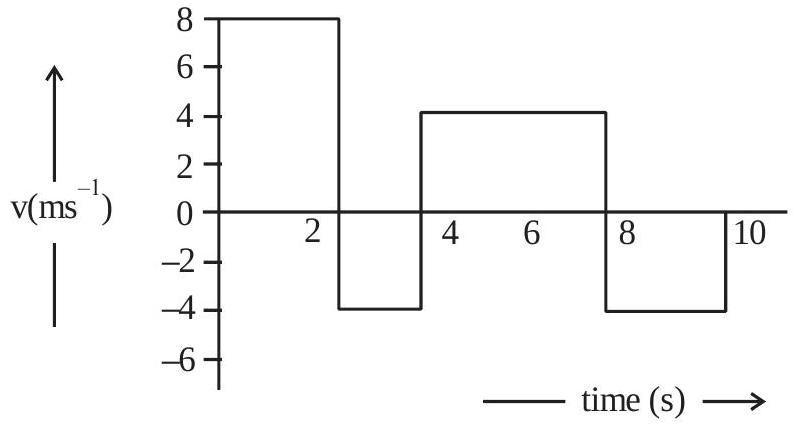
\includegraphics[max width=\textwidth, center]{2025_10_02_fdf5c730b8a604381ef3g-4(1)}

The ratio of displacement to distance travelled by the body in time 0 to 10 s is\\
(1) \(1: 1\)\\
(2) \(1: 4\)\\
(3) \(1: 2\)\\
(4) \(1: 3\)

Official Ans. by NTA (4)\\
Allen Ans. (4)\\
Sol. \(\quad\) Displacement \(=\) Darea \(=16-8+16-8=16 \mathrm{~m}\)\\
Distance \(=\Sigma \mid\) area \(\mid=48 \mathrm{~m}\)\\
\(\frac{\text { displacement }}{\text { Distan ce }}=\frac{1}{3}\)\\
16. Given below are two statements: one is labelled as

Assertion A and the other is labelled as Reason R\\
Assertion A: Steel is used in the construction of buildings and bridges.

Reason R: Steel is more elastic and its elastic limit is high.

In the light of above statements, choose the most appropriate answer from the options given below\\
(1) Both \(\mathbf{A}\) and \(\mathbf{R}\) are correct but \(\mathbf{R}\) is NOT the correct explanation of \(\mathbf{A}\)\\
(2) \(\mathbf{A}\) is not correct but \(\mathbf{R}\) is correct\\
(3) Both \(\mathbf{A}\) and \(\mathbf{R}\) are correct and \(\mathbf{R}\) is the correct explanation of \(\mathbf{A}\)\\
(4) \(\mathbf{A}\) is correct but \(\mathbf{R}\) is not correct

Official Ans. by NTA (3)\\
Allen Ans. (3)\\
Sol. Concept based\\
17. Given below are two statements: one is labelled as Assertion A and the other is labelled as Reason R. Assertion A: A pendulum clock when taken to Mount Everest becomes fast.

Reason R: The value of g (acceleration due to gravity) is less at Mount Everest than its value on the surface of earth.

In the light of the above statements, choose the most appropriate answer from the options given below\\
(1) Both \(\mathbf{A}\) and \(\mathbf{R}\) are correct but \(\mathbf{R}\) is NOT the correct explanation of \(\mathbf{A}\)\\
(2) Both \(\mathbf{A}\) and \(\mathbf{R}\) are correct and \(\mathbf{R}\) is the correct explanation of \(\mathbf{A}\)\\
(3) \(\mathbf{A}\) is not correct but \(\mathbf{R}\) is correct\\
(4) \(\mathbf{A}\) is correct but \(\mathbf{R}\) is not correct

Official Ans. by NTA (3)\\
Allen Ans. (3)\\
Sol. \(T \propto \frac{1}{\sqrt{g}}\)\\
18. A photon is emitted in transition from \(n=4\) to \(n=1\) level in hydrogen atom. The corresponding wavelength for this transition is\\
(given, \(\mathrm{h}=4 \times 10^{-15} \mathrm{eVs}\) ) :\\
(1) 94.1 nm\\
(2) 941 nm\\
(3) 97.4 nm\\
(4) 99.3 nm

Official Ans. by NTA (1)\\
Allen Ans. (1)\\
Sol. \(\frac{\mathrm{hc}}{\lambda}=\left[1-\frac{1}{16}\right](13.6 \mathrm{eV})\)\\
So, \(\lambda=94.1 \mathrm{~nm}\)\\
19. In an Isothermal change, the change in pressure and volume of a gas can be represented for three different temperature; \(T_{3}>T_{2}>T_{1}\) as :\\
(1)\\
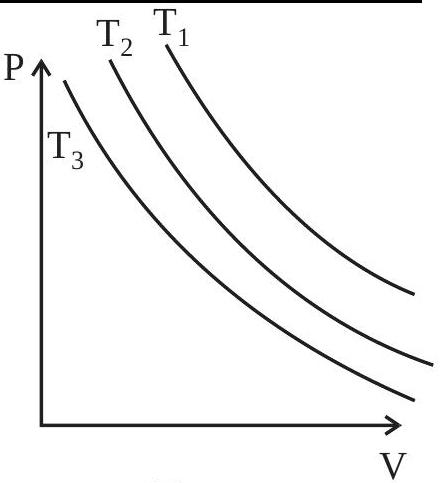
\includegraphics[max width=\textwidth, center]{2025_10_02_fdf5c730b8a604381ef3g-5}\\
(2)\\
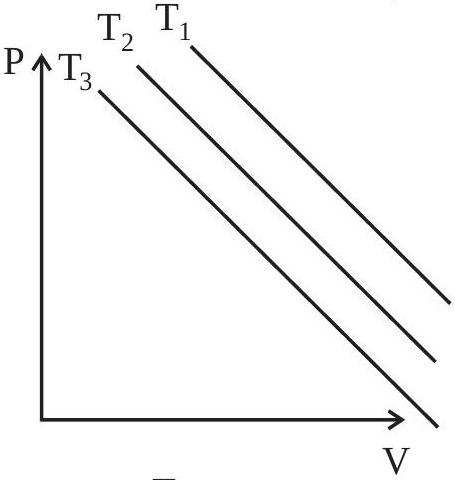
\includegraphics[max width=\textwidth, center]{2025_10_02_fdf5c730b8a604381ef3g-5(4)}\\
(3)\\
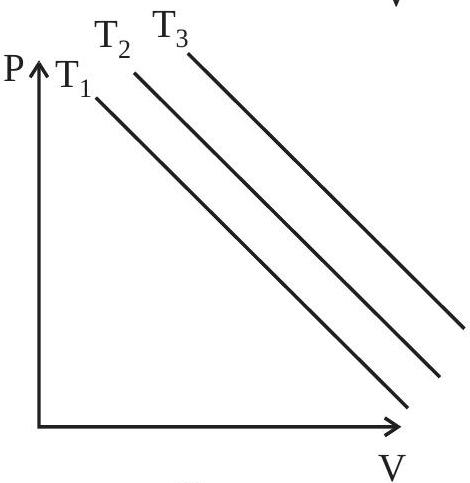
\includegraphics[max width=\textwidth, center]{2025_10_02_fdf5c730b8a604381ef3g-5(3)}\\
(4)\\
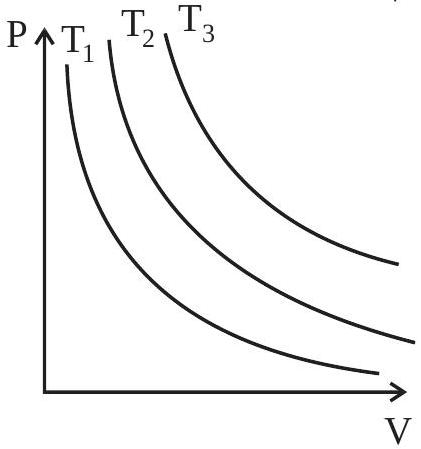
\includegraphics[max width=\textwidth, center]{2025_10_02_fdf5c730b8a604381ef3g-5(1)}

\section*{Official Ans. by NTA (4) \\
 Allen Ans. (4)}
Sol. For isothermal process P-V graph is rectangular hyperbola\\
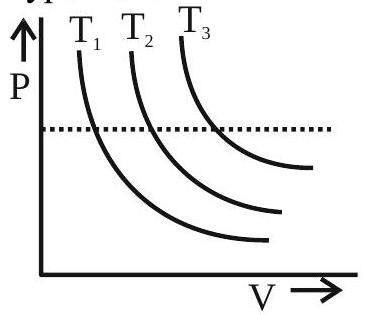
\includegraphics[max width=\textwidth, center]{2025_10_02_fdf5c730b8a604381ef3g-5(2)}

As dotted line is isobaric line which implies \(\mathrm{T}_{3}>\mathrm{T}_{2}>\mathrm{T}_{1}\) as volume is increasing.\\
20. If two vectors \(\overrightarrow{\mathrm{P}}=\hat{\mathrm{i}}+2 \mathrm{mj}+\mathrm{m} \hat{\mathrm{k}}\) and \(\overrightarrow{\mathrm{Q}}=4 \hat{\mathrm{i}}-2 \hat{\mathrm{j}}+\mathrm{m} \hat{\mathrm{k}}\) are perpendicular to each other. Then, the value of \(m\) will be :\\
(1) 1\\
(2) -1\\
(3) -3\\
(4) 2

Official Ans. by NTA (4)\\
Allen Ans. (4)\\
Sol. \(\overrightarrow{\mathrm{P}} \cdot \overrightarrow{\mathrm{Q}}=0\)\\
\((\hat{i}+2 m \hat{j}+m \hat{k}) \cdot(4 \hat{i}-2 \hat{j}+m \hat{k})=0\)\\
\(\Rightarrow 4-4 \mathrm{~m}+\mathrm{m}^{2}=0\)\\
\(\Rightarrow(\mathrm{m}-2)^{2}=0 \Rightarrow \mathrm{~m}=2\)

\section*{Section-B}
\begin{enumerate}
  \setcounter{enumi}{20}
  \item A uniform solid cylinder with radius \(R\) and length L has moment of inertia \(\mathrm{I}_{1}\), about the axis of cylinder. A concentric solid cylinder of radius \(R^{\prime}=\frac{R}{2}\) and length \(L^{\prime}=\frac{L}{2}\) is caned out of the original cylinder. If \(I_{2}\) is the moment of inertia of the carved out portion of the cylinder then \(\frac{\mathrm{I}_{1}}{\mathrm{I}_{2}}=\)\\
(Both \(\mathrm{I}_{1}\) and \(\mathrm{I}_{2}\) are about the axis of the cylinder)\\
Official Ans. by NTA (32)\\
Allen Ans. (32)\\
Sol.\\
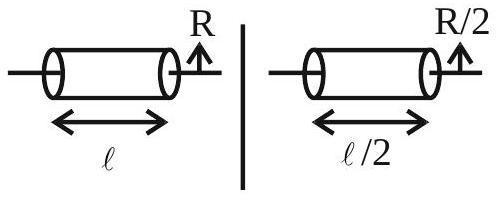
\includegraphics[max width=\textwidth, center]{2025_10_02_fdf5c730b8a604381ef3g-6}\\
\(\mathrm{I}_{1}=\frac{\mathrm{m}_{1} \mathrm{R}^{2}}{2} \quad \mathrm{I}_{2}=\frac{\mathrm{m}_{2}(\mathrm{R} / 2)^{2}}{2}\)\\
\(\frac{\mathrm{I}_{1}}{\mathrm{I}_{2}}=\frac{4 \mathrm{~m}_{1}}{\mathrm{~m}_{2}}=\frac{4 \cdot \rho \pi \mathrm{R}^{2} \ell}{\rho \cdot \frac{\pi \mathrm{R}^{2}}{4} \times \frac{\ell}{2}} \Rightarrow \frac{\mathrm{I}_{1}}{\mathrm{I}_{2}}=32\)
  \item A mass \(m\) attached to free end of a spring executes SHM with a period of 1 s . If the mass is increased by 3 kg the period of oscillation increases by one second, the value of mass \(m\) is \(\_\_\_\_\) kg.
\end{enumerate}

Official Ans. by NTA (1)\\
Allen Ans. (1)\\
Sol. \(\quad \mathrm{T}=2 \pi \sqrt{\frac{\mathrm{~m}}{\mathrm{k}}}=1\)\\
\(\mathrm{T}^{\prime}=2 \pi \sqrt{\frac{\mathrm{~m}+3}{\mathrm{k}}}=2\)\\
\(\frac{\mathrm{T}}{\mathrm{T}^{\prime}}=\sqrt{\frac{\mathrm{m}}{\mathrm{m}+3}}=\frac{1}{2}\)\\
\(\Rightarrow \frac{\mathrm{m}}{\mathrm{m}+3}=\frac{1}{4}\)\\
\(\mathrm{m}=1\)\\
23. The energy released per fission of nucleus of \({ }^{240} \mathrm{X}\) is 200 MeV . The energy released if all the atoms in 120 g of pure \({ }^{240} \mathrm{X}\) undergo fission is \(\_\_\_\_\) \(\times 10^{25}\) MeV .\\
(Given \(\mathrm{N}_{\mathrm{A}}=6 \times 10^{23}\) )\\
Official Ans. by NTA (6)\\
Allen Ans. (6)\\
Sol. No. of mole \(=\frac{120}{240}=\frac{1}{2}\)\\
No. of molecules \(=\frac{1}{2} \times \mathrm{N}_{\mathrm{A}}\)\\
Energy released \(=\frac{1}{2} \times 6 \times 10^{23} \times 200\)\\
\(=6 \times 10^{25} \mathrm{MeV}\)\\
24. A parallel plate capacitor with air between the plate has a capacitance of 15 pF . The separation between the plate becomes twice and the space between them is filled with a medium of dielectric constant 3.5. Then the capacitance becomes \(\frac{\mathrm{X}}{4} \mathrm{pF}\). The value of x is \(\_\_\_\_\) .

Official Ans. by NTA (105)\\
Allen Ans. (105)

Sol. \(\mathrm{C}_{0}=\frac{\in_{0} \mathrm{~A}}{\mathrm{~d}}=15 \mathrm{pF}\)\\
\(\mathrm{C}=\frac{\mathrm{K} \in_{0} \mathrm{~A}}{2 \mathrm{~d}}=\frac{3.5}{2} \times 15 \mathrm{pF}=\frac{105}{4} \mathrm{pF}\)\\
25. A body of mass 1 kg begins to move under the action of a time dependent force \(\overrightarrow{\mathrm{F}}=\left(t \hat{\mathrm{i}}+3 t^{2} \hat{\mathrm{j}}\right) \mathrm{N}\). where \(\hat{i}\) and \(\hat{j}\) are the unit vectors along \(x\) and \(y\) axis. The power developed by above force, at the time \(\mathrm{t}=2 \mathrm{~s}\). will be \(\_\_\_\_\) W.

Official Ans. by NTA (100)\\
Allen Ans. (100)\\
Sol. \(\overrightarrow{\mathrm{F}}=\mathrm{t} \hat{\mathrm{i}}+3 \mathrm{t}^{2} \hat{\mathrm{j}}\)\\
\(\frac{m d \vec{v}}{d t}=t \hat{i}+3 t^{2} \hat{j}\)\\
\(\mathrm{m}=1 \mathrm{~kg}, \int_{0}^{\vec{v}} \mathrm{dv}=\int_{0}^{\mathrm{t}} \mathrm{tdt} \hat{\mathrm{i}}+\int_{0}^{\mathrm{t}} 3 \mathrm{t}^{2} \mathrm{dt} \hat{\mathrm{j}}\)\\
\(\vec{v}=\frac{t^{2}}{2} \hat{i}+t^{3} \hat{j}\)\\
Power \(=\vec{F} \cdot \vec{V}=\frac{t^{3}}{2}+3 t^{5}\)

At \(\mathrm{t}=2\), power \(=\frac{8}{2}+3 \times 32\)\\
\(=100\)\\
26. If a copper wire is stretched to increase its length by \(20 \%\). The percentage increase in resistance of the wire is \(\_\_\_\_\) \(\%\).

Official Ans. by NTA (44)\\
Allen Ans. (44)\\
Sol. As volume is constant,\\
So resistance \(\propto(\text { length })^{2}\)\\
\(\Rightarrow \%\) change in resistance \(=20+20+\frac{400}{100}=44 \%\)\\
27. A single turn current loop in the shape of a right angle triangle with sides \(5 \mathrm{~cm}, 12 \mathrm{~cm}, 13 \mathrm{~cm}\) is carrying a current of 2 A . The loop is in a uniform magnetic field of magnitude 0.75 T whose direction is parallel to the current in the 13 cm side of the loop. The magnitude of the magnetic force on the 5 cm side will be \(\frac{x}{130} N\). The value of \(x\) is\\
\(\_\_\_\_\) .\\
Official Ans. by NTA (9)\\
Allen Ans. (9)\\
Sol.\\
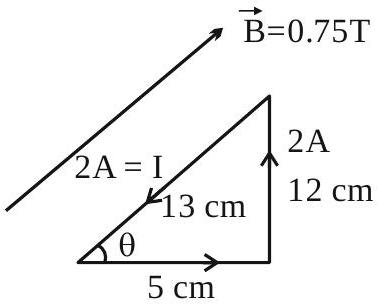
\includegraphics[max width=\textwidth, center]{2025_10_02_fdf5c730b8a604381ef3g-7}

Force on 5 cm side is\\
\(|\overrightarrow{\mathrm{F}}|=\mathrm{ILB} \sin \theta\)\\
\(=(2)\left(5 \times 10^{-2}\right) \times \frac{3}{4} \times \frac{12}{13}=\frac{9}{130} \mathrm{~N}\)\\
So, \(\mathrm{x}=9\)\\
28. Three identical resistors with resistance R = 12 , 2 , and two identical inductors with sell inductance \(\mathrm{L}=5 \mathrm{mH}\) are connected to an ideal battery with emf of 12 V as shown in figure. The current through the battery long after the switch has been closed will be \(\_\_\_\_\) A.\\
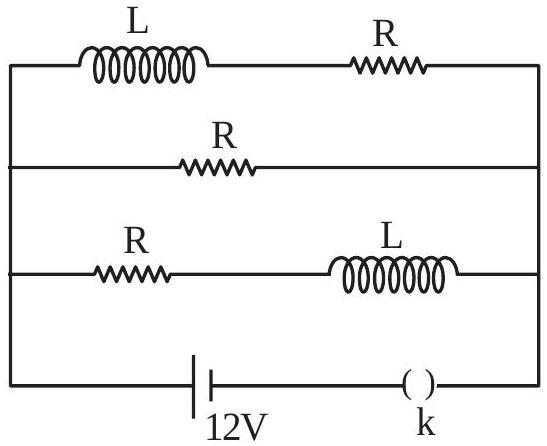
\includegraphics[max width=\textwidth, center]{2025_10_02_fdf5c730b8a604381ef3g-7(1)}

Official Ans. by NTA (3)\\
Allen Ans. (3)\\
Sol. After long time an inductor behaves as a resistance-less path.

So current through cell\\
\(\mathrm{I}=\frac{12}{\mathrm{R} / 3}=3 \mathrm{~A}\{\because \mathrm{R}=12 \Omega\}\)\\
29. A convex lens of refractive index 1.5 and focal length 18 cm in air is immersed in water. The change in focal length of the lens will be \(\_\_\_\_\) cm.\\
(Given refractive index of water \(=\frac{4}{3}\) )\\
Official Ans. by NTA (54)\\
Allen Ans. (54)\\
Sol. \(\frac{I}{f_{\mathrm{H}_{2} \mathrm{O}}}=\left(\frac{\mu_{\mathrm{g}}}{\mu_{\mathrm{H}_{2} \mathrm{O}}}-1\right)\left(\frac{2}{\mathrm{R}}\right)\)\\
\(=\frac{1}{8}\left(\frac{2}{\mathrm{R}}\right)\)\\
\(=\frac{1}{\left(4 \mathrm{f}_{\text {air }}\right)}\)\\
So, \(\mathrm{f}_{\mathrm{H}_{2} \mathrm{O}}=4 \mathrm{f}_{\text {air }}=72 \mathrm{~cm}\)\\
So change in focal length \(=72-18=54 \mathrm{~cm}\)\\
30. A Spherical ball of radius 1 mm and density \(10.5 \mathrm{~g} / \mathrm{cc}\) is dropped in glycerine of coefficient of viscosity 9.8 poise and density \(1.5 \mathrm{~g} / \mathrm{cc}\). Viscous force on the ball when it attains constant velocity is \(3696 \times 10^{-x} \mathrm{~N}\). The value of x is\\
(Given, \(\mathrm{g}=9.8 \mathrm{~m} / \mathrm{s}^{2}\) and \(\pi=\frac{22}{7}\) )\\
Official Ans. by NTA (7)\\
Allen Ans. (7)\\
Sol. When the ball attain terminal velocity\\
\(\mathrm{F}_{\mathrm{v}}=\left(\mathrm{mg}-\mathrm{F}_{\mathrm{B}}\right)(\because \mathrm{a}=0)\)\\
\(=V \sigma_{b} g-V \rho_{\ell} g\)\\
\(=\operatorname{Vg}\left(\sigma_{\mathrm{b}}-\rho_{\ell}\right)\)\\
\(=\frac{4}{3} \pi\left(10^{-3}\right)^{3} \times 9.8(10.5-1.5) \times 10^{3}\)\\
\(=3696 \times 10^{-7} \mathrm{~N}\)\\
So, \(\mathrm{x}=7\)


\end{document}